\subsubsection{Subproceso 3.B: Confirmaci\'on y Registro Oficial}

La Figura~\ref{fig:asis_3b_flujo} resume la secuencia horizontal del proceso actual. Empieza con la Pre-Ficha Aprobada o Subsanada que entrega el Subproceso 3.A: con ella el sistema bloquea la edici\'on antes disponible para el estudiante y registra su matr\'icula en el SIGA, sin tr\'amite adicional por la aprobaci\'on autom\'atica (TUPA PA5400954D, RR-3698-2024). En la semana de verificaci\'on se inscriben los rezagados y las rectificaciones de la primera semana (RR-0570-2022, Art. 77\textdegree{}) y se se\~nalan las electivas con menos de seis inscritos (RR-0570-2022, Art. 75\textdegree{}); el rombo de modificaciones extempor\'aneas recoge la solicitud que la Facultad presenta ante la DIRCE.

El proceso termina con el visado del Reporte y de la Boleta, los padrones para los docentes, el reporte externo y la devoluci\'on del registro a las Facultades.

La figura adem\'as marca el hallazgo del registro de campo del periodo 2026-2: la Facultad no puede editar la matr\'icula asentada, de modo que toda modificaci\'on extempor\'anea se tramita mediante solicitud ante la DIRCE. Los plazos del cierre, del reporte externo y de la devoluci\'on del registro ya est\'an descritos con las reglas del subproceso en la secci\'on 3. Las fuentes editables de ambas figuras se conservan en trabajo\_grupal/diagramas/ y se recompilan con PlantUML.

\begin{figure}[H]
    \centering
    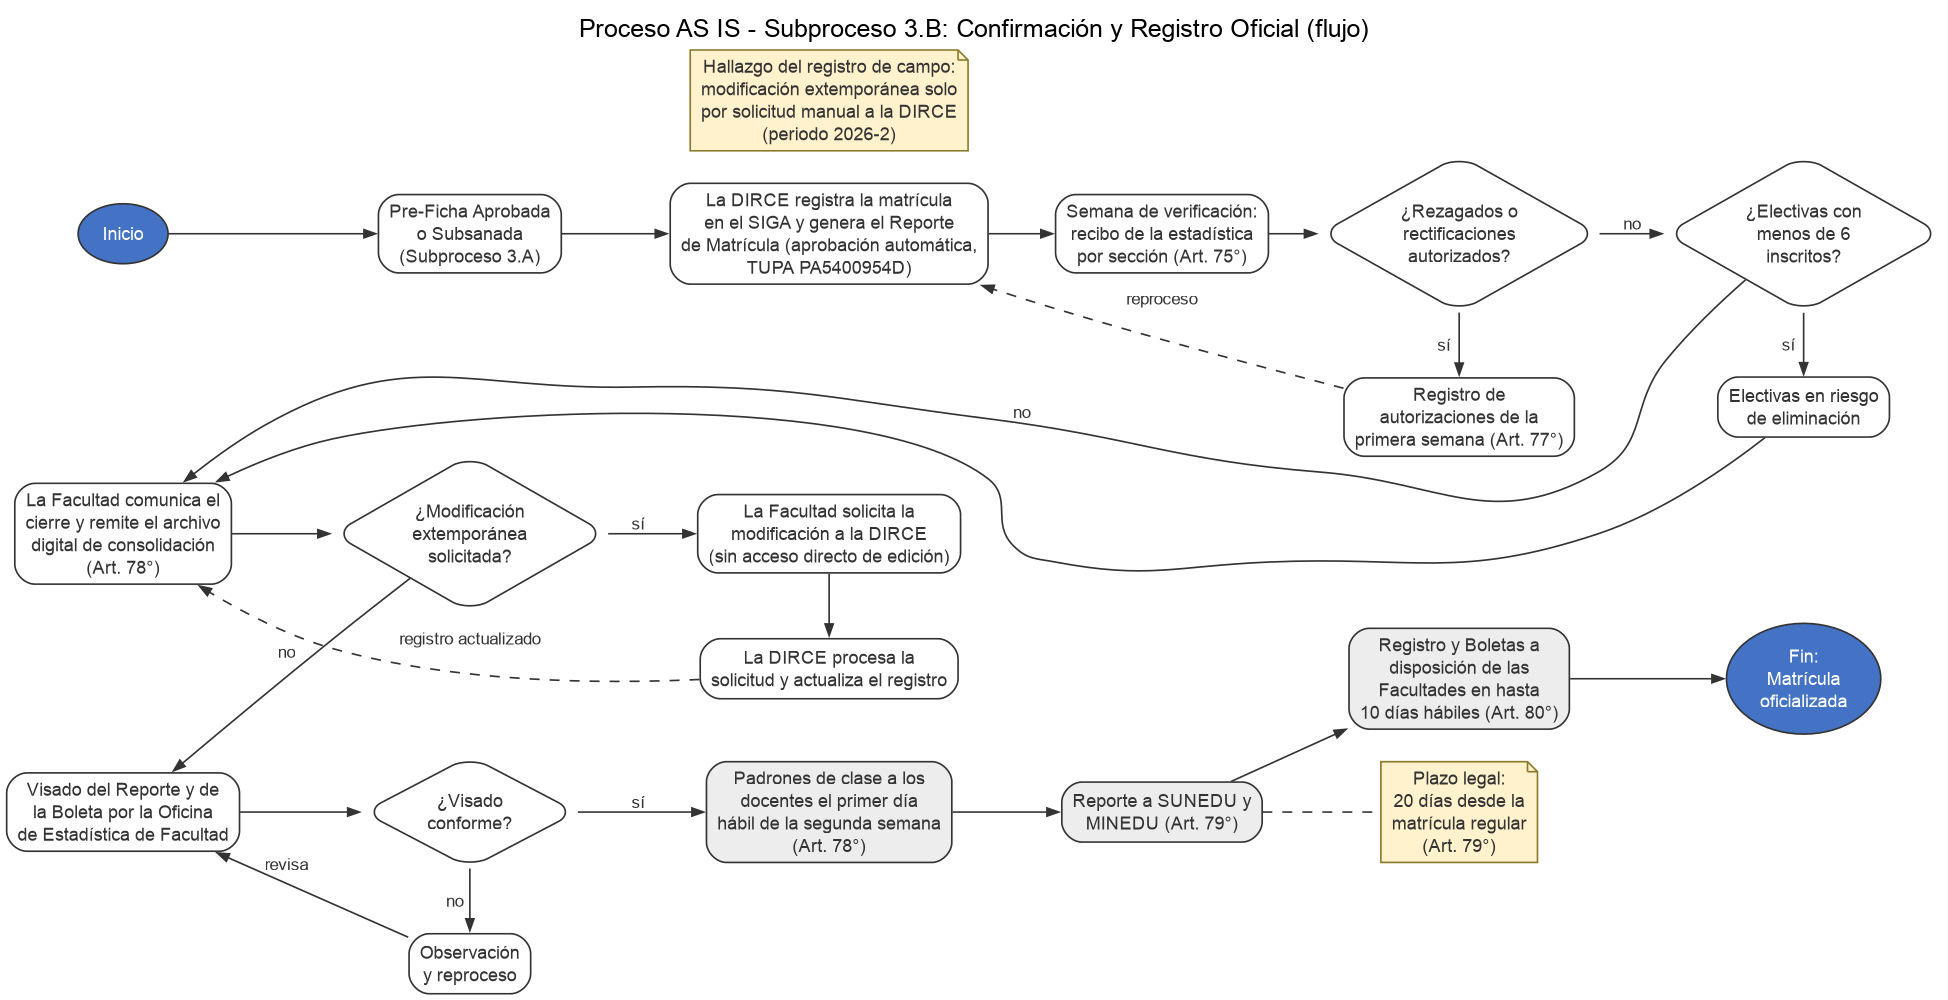
\includegraphics[width=0.95\textwidth]{asis_subproceso_3b_flujo.png}
    \caption{Diagrama de flujo (AS IS) del Subproceso 3.B}
    \label{fig:asis_3b_flujo}
\end{figure}

